\chapter{Marco teórico}
\label{ch:marco}

En este capítulo se presentan los conceptos teóricos que subyacen la propuesta de desarrollo de un conjunto de flujos de trabajo para la implementación de software embebido 
a bordo de computadoras de guía, navegación y control espacial. La información expuesta se deriva tanto de conocimientos propios como información bibliográfica.

\section{Estimación}
La estimación implica el uso de modelos matemáticos y algoritmos para calcular las variables de estado del sistema. Estas variables son esenciales para comprender 
el comportamiento del sistema y para tomar decisiones informadas sobre su control. La estimación puede realizarse de dos maneras:

\begin{itemize}
    \item Lazo abierto: En este enfoque, se utilizan modelos de estimación predefinidos sin retroalimentación, lo que significa que las estimaciones no se ajustan en función
    de las mediciones reales.
    \item Lazo cerrado: Este método ajusta las estimaciones en función de las mediciones reales y las salidas del sistema, lo que permite una mayor precisión y adaptabilidad.
\end{itemize}

Esta es crucial en aplicaciones donde las mediciones directas son difíciles o costosas de obtener, por ejemplo en los sistemas hidráulicos, la estimación de variables de 
estado permite optimizar el rendimiento y la eficiencia del sistema, asegurando que se mantengan las condiciones deseadas a pesar de las perturbaciones externas o errores en las 
mediciones \cite{Merchn2019EvaluacinDM}. La estimación es un componente clave en los sistemas de control, ya que facilita la comprensión y el manejo de sistemas complejos. 
Su implementación permite una operación más eficiente y efectiva, mejorando su capacidad de respuesta ante diversas condiciones operativas \cite{Mesa2020EstimacinDV}.

\section{Control}
La estimación es un componente clave en los sistemas de control, ya que este se enfoca en el diseño y desarrollo de sistemas capaces de regular y controlar variables de un proceso de manera autónoma. Estos sistemas utilizan sensores, actuadores y algoritmos de control para mantener las variables de interés dentro de los rangos permitidos, mejorando de esta forma la eficiencia, precisión y confiabilidad de los procesos. Su aplicación abarca desde sistemas espaciales hasta sistemas de iluminación. 


\section{Procesadores embebidos}

Los procesadores embebidos están especializados en tareas dentro de un sistema más complejo. A diferencia de los procesadores de propósito general, están 
optimizados para ofrecer eficiencia energética, un tamaño compacto y costo reducido. Algunas de las características de los procesadores embebidos son:

\begin{itemize}
    \item Integración de periféricos: Incorporan periféricos específicos de la aplicación en un único chip, incluyendo temporizadores, puertos de entrada/salida y controladores 
    de memoria.
    \item Arquitecturas de bajo Consumo: Diseñados para maximizar la duración de la batería en dispositivos portátiles, lo que es esencial para la operatividad de dispositivos 
    móviles.
    \item Tamaño compacto: Su diseño permite reducir costos y facilitar la integración en espacios limitados, lo que los hace ideales para aplicaciones donde el espacio es 
    crítico.
    \item Capacidad de respuesta en tiempo real: Pueden responder a eventos externos de manera predecible y determinista, lo que es crucial en aplicaciones que requieren una respuesta rápida y precisa.
\end{itemize}

\subsection{Cortex-A9}

Los procesadores embebidos basados en la arquitectura ARM Cortex-A9 se utilizan en aplicaciones de alto rendimiento y capacidades avanzadas de procesamiento.
Aunque esta arquitectura no es un procesador embebido, sino más bien una familia de núcleos de procesador diseñado por ARM Holdings, los sistemas en chip que incorporan
estos núcleos han demostrado ser una solución popular para aplicaciones embebidas \cite{Schwiegelshohn2014DesignOA}. Algunas de sus características son: 

\begin{itemize}
    \item Arquitectura de 32 bits basada en ARM v7-A.
    \item Alto rendimiento adecuado para aplicaciones exigentes como sistemas operativos embebidos, procesamiento multimedia y gráficos.
    \item Características avanzadas como unidades de coma flotante, unidades de procesamiento NEON para procesamiento multimedia y soporte para virtualización.
\end{itemize}

Algunos sistemas en chip que incorporan núcleos Cortex-A9 son:

\begin{itemize}
    \item Nvidia Tegra 3: Combina cuatro núcleos Cortex-A9 y una GPU.
    \item Texas Instruments OMAP 4: Familia de sistemas en chip que combina núcleos Cortex-A9 y DSP.
    \item Xilinx Zynq-7000: Integra núcleos Cortex-A9 con lógica programable FPGA.
\end{itemize}

\subsection{Tarjeta de desarrollo ZedBoard}

La ZedBoard es una tarjeta de desarrollo basada en el Xilinx Zynq-7000 la cual integra núcleos Cortex-A9 con la lógica programable para Field Programmable Gate Array, por sus siglas en ingles (FPGA). Esta plataforma es ideal para prototipar aplicaciones en el ámbito de sistemas embebidos. La tabla \ref{tab:zedboard} resume las especificaciones que posee la tarjeta de desarrollo ZedBoard.


\begin{figure}[h!]
    \centering
    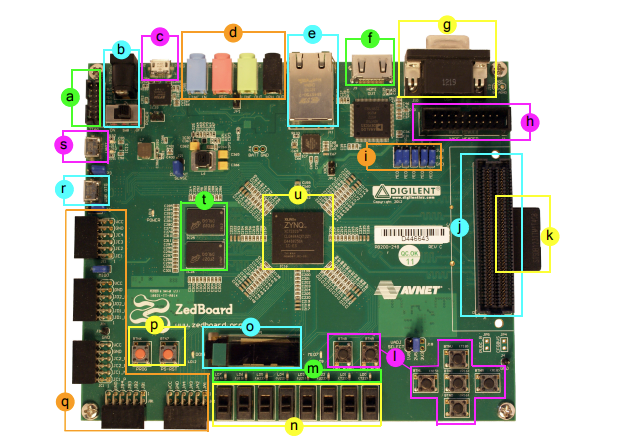
\includegraphics[width=0.8\textwidth]{fig/teorico/zedboard_raw.png}
    \caption{Tarjeta de desarrollo ZedBoard}
    \label{fig:zedboard_raw_info}
\end{figure}

Como se observó en \ref{fig:zedboard_raw_info}, esta tarjeta de desarrollo cuenta con los puertos de conexión que se mencionan en la Tabla \ref{tab:puertos_yocto}: 

\begin{table}[htbp!]
    \caption{Puertos de entrada y salida de la plataforma de desarrollo Zedbord}
    \label{tab:puertos_yocto}
    \resizebox{\textwidth}{!}{%
    \begin{tabular}{|l|l|ll}
    \hline
    Identificador & Descripción                     & \multicolumn{1}{l|}{Identificador} & \multicolumn{1}{l|}{Descripción}      \\ \hline
    a             & Conector JTAG Xilinx            & \multicolumn{1}{l|}{l}             & \multicolumn{1}{l|}{Pulsadores}       \\ \hline
    b & Entrada de voltaje e   interruptor de encendido & \multicolumn{1}{l|}{m} & \multicolumn{1}{l|}{LED}                                 \\ \hline
    c             & USB-JTAG para   programación    & \multicolumn{1}{l|}{n}             & \multicolumn{1}{l|}{Interruptores}    \\ \hline
    d             & Puertos de audio                & \multicolumn{1}{l|}{o}             & \multicolumn{1}{l|}{Pantalla OLED}    \\ \hline
    e & Puerto de Ethernet                              & \multicolumn{1}{l|}{p} & \multicolumn{1}{l|}{Botones de   programación y reinicio} \\ \hline
    f             & Puerto HDMI (Salida   de video) & \multicolumn{1}{l|}{q}             & \multicolumn{1}{l|}{Conectores Pmod}  \\ \hline
    g & Puerto VGA (Salida de   video)                  & \multicolumn{1}{l|}{r} & \multicolumn{1}{l|}{USB OTG para   periféricos}           \\ \hline
    h             & Puerto XADC                     & \multicolumn{1}{l|}{s}             & \multicolumn{1}{l|}{USB UART}         \\ \hline
    i             & Puentes  de   configuración      & \multicolumn{1}{l|}{t}             & \multicolumn{1}{l|}{Memoria DDR3}     \\ \hline
    j             & Conector FCM                    & \multicolumn{1}{l|}{u}             & \multicolumn{1}{l|}{Dispositivo Zynq} \\ \hline
    k             & Entrada para tarjeta   SD       &                                    &                                       \\ \cline{1-2}
    \end{tabular}%
    }
\end{table}

\begin{table}[h!]
    \caption{Especificaciones generales de la tarjeta de desarrollo ZeadBoard}
    \label{tab:zedboard}
    \resizebox{\textwidth}{!}{%
    \begin{tabular}{|l|l|}
    \hline
    \multicolumn{1}{|c|}{\textbf{Especificación}} & \multicolumn{1}{c|}{\textbf{Detalles}} \\ \hline
    \textbf{Procesador}             & Xilinx Zynq-7000 (XC7Z020)                         \\ \hline
    \textbf{Núcleos de Procesador}  & ARM Cortex-A9 de doble núcleo                      \\ \hline
    \textbf{Memoria DDR3}           & 512 MB                                             \\ \hline
    \textbf{Memoria Flash}          & 256 MB QSPI                                        \\ \hline
    \textbf{Almacenamiento}         & Tarjeta SD de 4 GB                                 \\ \hline
    \textbf{Conectividad}           & Ethernet (10/100/1000 Mbps), USB OTG 2.0, USB-UART \\ \hline
    \textbf{Salidas de Video}       & HDMI (1080p), VGA de 8 bits, OLED 128x32           \\ \hline
    \textbf{Audio}                  & Códec de audio I2S                                 \\ \hline
    \textbf{Puertos GPIO}           & 54 pines GPIO                                      \\ \hline
    \textbf{Interfaz de JTAG}       & Soporte para programación y depuración             \\ \hline
    \textbf{Dimensiones}            & 10.2 cm x 6.4 cm                                   \\ \hline
    \textbf{Fuente de Alimentación} & 5V a través de conector de alimentación            \\ \hline
    \textbf{Sistema Operativo}      & Soporte para Linux y otros sistemas embebidos      \\ \hline
    \textbf{Expansión}              & Conectores Pmod y FMC para módulos adicionales     \\ \hline
    \end{tabular}%
    }
\end{table}

Además de esto algunas especificaciones de la plataforma de desarrollo se mencionan en la Tabla \ref{tab:zedboard}. Por otro lado la ZedBoard es una plataforma de desarrollo altamente versátil que se destaca por su capacidad para ejecutar sistemas operativos como Linux, lo que la convierte en una opción ideal para proyectos de diseño y desarrollo de sistemas embebidos. Además de su compatibilidad con Linux, la ZedBoard cuenta con especificaciones técnicas que la hacen destacar en el ámbito del desarrollo. Entre ellas se incluyen un procesador ARM Cortex-A9. 

\section{Marcos de trabajo}

Los marcos de trabajo en sistemas embebidos son conjuntos de herramientas y bibliotecas que facilitan el desarrollo de aplicaciones en estos 
sistemas. Proporcionan una estructura que permite abordar los desafíos específicos que presentan los sistemas embebidos.

Los sistemas embebidos interactúan con su entorno físico, lo que requiere un diseño que no solo considere los resultados de las operaciones, sino también el cumplimiento de plazos y restricciones específicas. En este contexto, las propiedades no funcionales, como el consumo energético, la latencia, la fiabilidad y el manejo de recursos, son críticos para el diseño y optimización del rendimiento general del sistema \cite{Marugn2017SimulacinYV}. Los marcos de trabajo juegan un papel fundamental al proporcionar herramientas y bibliotecas predefinidas, permitiendo a los desarrolladores centrarse en la lógica de la  aplicación en lugar de lidiar con los detalles de bajo nivel del hardware, lo que acelera el proceso de desarrollo y reduce la posibilidad de errores. 

Algunos ejemplos de marcos de trabajo populares en sistemas embebidos incluyen Robot Operating System (ROS), utilizado en aplicaciones de robótica, y FreeRTOS, un sistema operativo de tiempo real diseñado para microcontroladores y sistemas embebidos \cite{HerreraLpez2023EntornoDT}.

\subsection{Yocto Project}\label{subsec:yocto}

Yocto es un marco de trabajo o bien del inglés (Framework) popular utilizado en el desarrollo de sistemas embebidos, especialmente en la creación de distribuciones de Linux personalizadas para hardware específico. Yocto utiliza un proceso de construcción cruzada, lo que significa que el código se compila en una plataforma diferente a la que se ejecutará, permitiendo que el código se optimice para el hardware específico del sistema embebido \cite{Leppakoski2013FrameworkFI}.

\begin{figure}[h!]
    \centering
    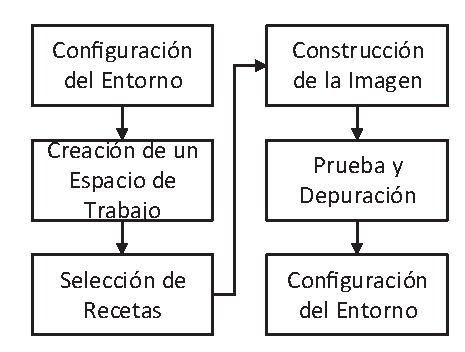
\includegraphics[width=0.5\textwidth]{fig/teorico/Flujo de trabajo de yocto.pdf}
    \caption{Flujo de trabajo Yocto Project}
    \label{fig:yocto_project_workflow}
\end{figure}

Una de las principales ventajas de Yocto es su flexibilidad en la configuración del sistema, permitiendo a los desarrolladores seleccionar paquetes específicos, configurar algunas opciones de compilación y personalizar el sistema operativo según sus necesidades. Además, Yocto fomenta la reutilización de código a través de capas, que son colecciones de recetas, configuraciones y parches que se pueden agregar o eliminar fácilmente del flujo de trabajo en construcción \cite{Leppakoski2013FrameworkFI}.

\section{MATLAB}
MATLAB es un software de cálculo técnico desarrollado por MathWorks, ampliamente utilizado en diversas áreas de la ciencia y la ingeniería. Proporciona un entorno interactivo para el desarrollo de algoritmos, análisis de datos, visualización y cálculo numérico. Su facilidad para trabajar con vectores y matrices lo distingue de otros sistemas de cálculo \cite{PealozaLuna2022SimulacinDU}. Es comúnmente utilizado para simular sistemas eléctricos, como convertidores DC/DC, y realizar análisis numéricos en problemas complejos \cite{OrdezGarca2022MatlabCU}. 

MATLAB juega un papel crucial en el desarrollo de sistemas de control aeroespaciales, facilitando la simulación, modelado y control de vehículos aéreos no tripulados (UAV) y otros sistemas relacionados. MATLAB, junto con Simulink, permite el modelado cinemático y dinámico de UAVs. Esto incluye la programación y control de sus movimientos, como cabeceo, utilizando motores de corriente directa y codificadores ópticos para medir su posición \cite{Senz2020LaboratorioPE} \cite{ChvezGudio2023DesarrolloYC}.

\subsection{Simulink}

Simulink, es un entorno de simulación y diseño gráfico que forma parte del software MATLAB. Se utiliza principalmente para modelar, simular y analizar sistemas dinámicos, especialmente aquellos que involucran componentes eléctricos, mecánicos y de control, algunas  de las características principales de Simulink son:

\begin{itemize}
    \item Modelado Gráfico
    \item Simulación en Tiempo real
    \item Integración con MATLAB
    \item Diseño de Controladores
    \item Análisis de Sistemas Dinámicos
\end{itemize}

Es una herramienta que permite a los usuarios crear modelos visuales de sistemas complejos utilizando bloques representativos, facilitando así su diseño y comprensión. Ofrece simulaciones en tiempo real, esenciales para la evaluación del comportamiento de sistemas en ingeniería y control bajo diversas condiciones \cite{PealozaLuna2022SimulacinDU}. Su integración con MATLAB potencia las capacidades de análisis y programación, permitiendo un análisis más profundo y la personalización de simulaciones \cite{Daza2021PlataformaDP}. Simulink se aplica en diversas áreas como la ingeniería eléctrica, mecánica, robótica y diseño de sistemas de control, siendo especialmente útil para diseñar y probar controladores, analizar sistemas dinámicos y desarrollar prototipos rápidos para sistemas embebidos \cite*{CardozoSarmiento2019SimulationOI}.

\section{Transformación de modelo a modelo}\label{sec:modelo2model}

La transformación de modelo a modelo hace referencia a un proceso en el que un modelo se convierte en otro, manteniendo la esencia de su estructura y funcionalidad, pero adaptándose a nuevas necesidades o contextos. Este concepto es fundamental en la Ingeniería de Software, especialmente dentro de la Arquitectura Dirigida por Modelos (MDA), donde se busca facilitar la interoperabilidad y la portabilidad de sistemas a través de la transformación de modelos independientes de la computación 
(CIM) a modelos independientes de la plataforma (PIM) y viceversa.

\begin{itemize}
    \item Modelos de Datos a Modelos de Aplicación:
    \item Modelos de Negocio a Modelos de Implementación
    \item Modelos UML a Código Fuente
\end{itemize}

Para efectos de este trabajo el área de interés serán la transformación de UML a Código Fuente.

%\subsection{MATLAB Embedded Coder}
%
%El MATLAB Embedded Coder se adapta a esta definición de transformación de modelo a modelo, ya que permite a los usuarios generar código C y C++ a partir de modelos Simulink. Esto es especialmente %útil en el desarrollo de sistemas embebidos, donde se requiere que los modelos de alto nivel se transformen en código que pueda ser ejecutado en hardware específico. Esta herramienta facilita la %implementación de algoritmos y sistemas de control, asegurando que el modelo original se traduzca eficazmente en un formato que pueda ser utilizado en entornos de producción.

\subsection{MATLAB Simulink Coder}

Simulink Coder es una herramienta del entorno MATLAB/Simulink que permite generar automáticamente código C y C++ a partir de modelos gráficos, facilitando la implementación de algoritmos en hardware o software. Sus características incluyen la generación de código automática, integración con diversas plataformas de hardware, optimización del rendimiento y soporte para modelos complejos, lo que la hace ideal para aplicaciones en control de sistemas, simulación y pruebas, y desarrollo ágil. En resumen, Simulink Coder es esencial para transformar modelos teóricos en aplicaciones prácticas, mejorando tanto el proceso de desarrollo como el rendimiento del producto final.


\begin{figure}[h!]
    \centering
    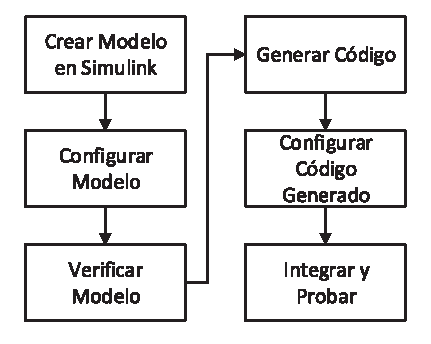
\includegraphics[width=0.45\textwidth]{fig/teorico/Flujo de trabajo simulink coder.pdf}
    \caption{Flujo de trabajo Simulink Coder}
    \label{fig:Simulink_coder_workflow}
\end{figure}

Como se observa en la Figura \ref{fig:Simulink_coder_workflow}, primeramente se debe de diseñar el modelo utilizando bloques de Simulink para representar el sistema o algoritmo a implementar, una vez generado el diagrama se deben de ajustar las configuraciones del modelo, incluyendo parámetros como el tipo de solución, la frecuencia de muestreo y las opciones de simulación, además de esto se deben de realizar simulaciones para verificar que el modelo funcione correctamente y cumpla con los requisitos especificados. 

Finalmente se debe de hacer uso de la herramienta Simulink Coder para generar automáticamente código C o C++ a partir del modelo validado. Adicionalmente a este código generado se pueden realizar configuraciones según se desea su ejecución, estas configuraciones son opciones adicionales para la generación del código, como optimización y estilo de codificación. Una vez aplicados todos los cambios necesarios se debe integrar el código generado en un entorno de desarrollo adecuado y realizar pruebas para asegurar que el código se comporta como se espera en el hardware objetivo.

\section{Código embebido}

El código embebido es un tipo de software diseñado para operar en dispositivos con recursos limitados, como microcontroladores y sistemas embebidos. Este código es fundamental en la programación de dispositivos electrónicos, permitiendo que estos realicen tareas específicas, como gestionar un sistema de automatización industrial o incluso operar en dispositivos móviles. Se caracteriza por su ejecución en dispositivos con recursos limitados, su capacidad para controlar dispositivos electrónicos, el uso de lenguajes de bajo nivel, la optimización de recursos y la necesidad de garantizar tiempos de respuesta 
determinísticos.

\section{Compilación Cruzada}

Es un proceso clave en el desarrollo de software que permite compilar código fuente en un sistema operativo o arquitectura de hardware diferente al utilizado para el desarrollo. Este método es especialmente valioso en entornos como sistemas embebidos, donde la plataforma de destino no es adecuada para la compilación directa. Utiliza compiladores específicos, conocidos como compiladores cruzados, que generan código ejecutable para la plataforma de destino desde una plataforma de origen. Esto permite a los desarrolladores trabajar en sus máquinas locales, como Windows o Linux, mientras crean aplicaciones para dispositivos como microcontroladores o sistemas operativos variados.

Además de su uso en sistemas embebidos, la compilación cruzada es fundamental para el desarrollo multiplataforma, ya que facilita la creación de aplicaciones que funcionan en diferentes sistemas operativos sin necesidad de modificar el código base. Este enfoque no solo mejora la eficiencia del proceso de desarrollo y pruebas, sino que también evita la constante transferencia de código a la plataforma de destino. 

En resumen, la compilación cruzada es una técnica esencial en el desarrollo moderno de software, permitiendo abordar múltiples plataformas y arquitecturas con mayor facilidad.

\begin{figure}[h!]
    \centering
    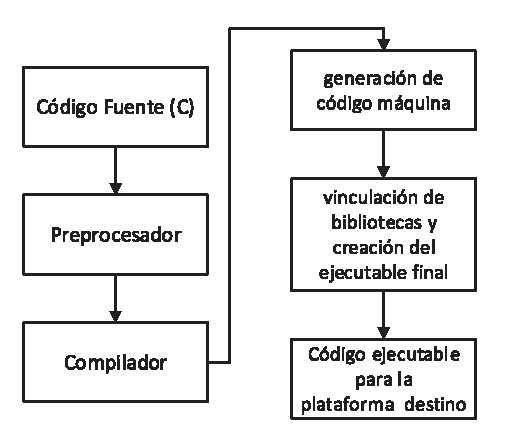
\includegraphics[width=0.5\textwidth]{fig/teorico/Flujo de trabajo xcompiler.pdf}
    \caption{Diagrama de compilación cruzada}
    \label{fig:xcompile_workflow}
\end{figure}

La Figura \ref{fig:xcompile_workflow}, nos demuestra como el proceso de compilación de un programa en lenguaje C comienza con el código fuente, que es el conjunto de instrucciones escritas por el programador. Después, se utiliza el preprocesador, que lleva a cabo tareas esenciales como la inclusión de archivos y la expansión de macros, generando un archivo intermedio que está listo para ser compilado. Posteriormente, el compilador analiza este archivo intermedio y produce código objeto, una representación en lenguaje máquina que aún no está completamente vinculada. Este código objeto es luego procesado por el ensamblador, que lo convierte en código máquina, específico para la arquitectura del sistema objetivo.

\section{Contenedores}\label{sec:containers}

Los contenedores en software son una tecnología que permite empaquetar aplicaciones junto con todas sus dependencias en un entorno aislado y portable. Esto asegura que la aplicación funcione de manera consistente en diferentes entornos, desde la máquina de desarrollo hasta los servidores de producción.

\subsection{Docker}

Docker ha revolucionado la forma en que se desarrollan y despliegan aplicaciones al ofrecer un entorno portátil y consistente. Gracias a su capacidad de empaquetar aplicaciones junto con todas sus dependencias, los desarrolladores pueden estar seguros de que su software funcionará de manera idéntica en cualquier entorno, ya sea local, en la nube o en producción. Esta portabilidad no solo ahorra tiempo en la configuración del entorno, sino que también reduce significativamente los problemas relacionados con "funciona en mi máquina". Además, el aislamiento que proporcionan los contenedores asegura que las aplicaciones operen sin interferencias, lo que es crucial para mantener la estabilidad y el rendimiento.

Por otro lado, la eficiencia de Docker es notable. A diferencia de las máquinas virtuales, los contenedores comparten el núcleo del sistema operativo, lo que permite un uso más optimizado de los recursos y un inicio casi instantáneo. Esto se traduce en una mayor agilidad y rapidez al escalar aplicaciones, ya que se pueden crear y gestionar múltiples instancias de contenedores con facilidad. La capacidad de versionar imágenes también es un gran beneficio, ya que permite a los equipos mantener un historial claro de cambios y revertir a versiones anteriores cuando sea necesario. En conjunto, estas características hacen de Docker una herramienta indispensable para la integración y entrega continua (CI/CD), mejorando significativamente los flujos de trabajo de desarrollo y despliegue.

\section{Protocolos de Comunicación}\label{sec:protocolos_de_comunicacion}

Los protocolos de comunicación son un conjunto de reglas y convenciones que permiten la transmisión de datos entre dispositivos en una red. Estos protocolos son esenciales para garantizar que los dispositivos puedan intercambiar información de manera efectiva y segura \cite{Eterovic2018AnlisisDP}.

\subsection{UART}

El protocolo receptor-transmisor asíncrono universal por sus siglas en ingles (UART) es un protocolo de comunicación serial ampliamente utilizado para la transmisión de datos entre dispositivos. Su característica principal es ser asíncrono, lo que significa que no requiere una señal de reloj compartida entre el transmisor y el receptor.

\textbf{Características:}

\begin{itemize}
    \item Transmisión Asíncrona: No necesita sincronización de reloj, lo que simplifica su implementación y reduce la complejidad del sistema.
    \item Configuración Simple: Opera comúnmente con configuraciones de 8 bits de datos, 1 bit de parada y 1 bit de paridad opcional, facilitando su uso en diversas aplicaciones.
    \item Distancia de Comunicación: Es efectivo para distancias cortas, generalmente menos de 15 metros, debido a la posible degradación de la señal a medida que aumenta la distancia.
    \item Velocidad de Transmisión: Las tasas de baudios (baud rate) pueden variar desde 300 hasta 115200 bps o más, dependiendo del hardware y las condiciones del entorno.
\end{itemize}

\textbf{Aplicaciones:}

\begin{itemize}
    \item Comunicación entre microcontroladores.
    \item Interfaces para sensores y dispositivos periféricos.
    \item Envío de datos a través de puertos serie en computadoras y dispositivos embebidos.
\end{itemize}

\subsection{SSH}

El Secure Shell por sus siglas en ingles (SSH), es un protocolo de red que permite la administración segura de dispositivos y la transferencia de datos a través de redes inseguras. SSH proporciona autenticación y cifrado, garantizando que los datos transmitidos estén protegidos contra ataques maliciosos.

\textbf{Características:}

\begin{itemize}
    \item Cifrado: Utiliza algoritmos de cifrado robustos, como AES, para proteger la información durante su transmisión.
    \item Autenticación: Permite autenticación mediante contraseña o claves públicas, aumentando significativamente la seguridad en el acceso a los sistemas.
    \item Túneles Seguros: Facilita la creación de túneles seguros para otros protocolos, lo que permite la transferencia protegida de datos sensibles.
    \item Interfaz de Línea de Comando: Proporciona acceso remoto a la línea de comandos, permitiendo a los administradores gestionar sistemas sin necesidad de estar físicamente presentes.
\end{itemize}

\section{Computadoras de guía, navegación y control}

Las computadoras de guía, navegación y control son esenciales en diversas aplicaciones, particularmente en aviación, navegación marítima y vehículos autónomos. Su función principal radica en procesar datos de sensores para ofrecer información precisa que facilite la toma de decisiones en tiempo real. Estas tecnologías son fundamentales para garantizar la seguridad y eficiencia en el transporte moderno.

Existen tres tipos principales de computadoras en este ámbito: las computadoras de navegación, que determinan la posición y rumbo de embarcaciones o aeronaves mediante sistemas GPS e inerciales; las computadoras de control, que regulan el movimiento y estabilidad de los vehículos, como los controladores de vuelo; y las computadoras de guía, que ofrecen rutas óptimas a través de sistemas de navegación por satélite. Los componentes clave incluyen sensores que recogen datos del entorno, procesadores que realizan cálculos complejos e interfaces de usuario que permiten la interacción con el sistema.

Las aplicaciones de estas computadoras son variadas y críticas. En la aviación, se utilizan para el control de vuelo en aeronaves comerciales y militares. En la navegación marítima, aseguran rutas seguras para barcos. Además, son integradas en vehículos autónomos como coches y drones, permitiendo una navegación eficiente sin intervención humana. En conjunto, estas tecnologías no solo mejoran la seguridad, sino que también optimizan la eficacia del transporte actual.

\subsection{EXA ICEPS}\label{sec:exaiceps}
La computadora de vuelo EXA ICEPS (Integrated Control and Engine Performance System) es una tecnología avanzada diseñada para gestionar y optimizar el rendimiento del motor y otros sistemas críticos en aeronaves. Su integración de sistemas permite combinar el control del motor con diferentes funciones de la aeronave, lo que resulta en una gestión más eficiente y segura durante el vuelo.

Entre sus principales características se destacan el monitoreo en tiempo real, que proporciona datos sobre el rendimiento del motor, permitiendo a los pilotos tomar decisiones informadas. Además, la EXA ICEPS optimiza el rendimiento al maximizar la eficiencia del combustible y reducir las emisiones, contribuyendo así a operaciones más sostenibles. Sus funciones incluyen el control automático de los parámetros del motor, la facilitación del diagnóstico y mantenimiento predictivo, lo que ayuda a reducir costos operativos.

Este sistema ejemplifica cómo la tecnología moderna está revolucionando la aviación, mejorando tanto la seguridad como la eficiencia operativa. Al integrar múltiples funciones y proporcionar información crítica en tiempo real, la EXA ICEPS no solo optimiza el rendimiento de las aeronaves, sino que también promueve prácticas más sostenibles en la industria.

\section{Revisión literaria}
En los últimos años, las computadoras de guía, navegación y control han mostrado grandes avances en el desarrollo de sistemas autónomos.

\subsection{Desarrollo de sistemas de navegación}

En 2022, se presentó un sistema de planificación y control de navegación para vehículos autónomos en entornos urbanos. Este sistema permite la planificación 
de rutas basadas en la posición actual del vehículo y su destino, utilizando un controlador clásico que asegura el seguimiento de la trayectoria mediante 
odometría y correcciones visuales. Los resultados se simularon utilizando herramientas como ROS y Gazebo, lo que demuestra la viabilidad de estos sistemas en 
entornos complejos \cite{BarreraRamrez2022SistemaDP}. 

\subsection{Transformación de Lenguaje de Bloques a Código C}

La traducción de código de control de lenguaje de bloques a C implica un proceso de conversión donde cada bloque visual se asocia con una estructura de código 
en C. Esto se puede hacer utilizando herramientas de software que generan automáticamente el código C a partir de la lógica definida en el entorno de bloques. 
Este proceso no solo facilita la programación, sino que también permite la optimización del código generado para mejorar el rendimiento en sistemas de navegación 
autónoma.

\subsubsection{XOD}

XOD es un entorno de programación visual basado en bloques que permite a los usuarios crear programas para microcontroladores como Arduino. Este software 
genera automáticamente código en C++ a partir de la lógica definida en bloques. Los usuarios pueden conectar componentes gráficamente y, al finalizar, acceder 
al código generado, que es abierto y personalizable. XOD es gratuito y permite la creación de nuevos nodos para componentes específicos, lo que facilita la 
adaptación a diferentes proyectos \cite{Snchez2020ProgramacinDL}.

\subsubsection{Visual Microcontroller}
Este software proporciona un lenguaje de programación gráfico para microcontroladores, desarrollado en C\#. Utiliza una interfaz gráfica que permite a los 
usuarios diseñar diagramas que representan la lógica de control. El sistema compila el código a partir de diagramas gráficos, generando código intermedio 
en C antes de llegar al código hexadecimal necesario para la programación del microcontrolador \cite{Sacta2011DesarrolloDU}.

\subsubsection{Simulink}
Como se mencionó anteriormente, Simulink, parte de MATLAB, proporciona un entorno gráfico para modelar, simular y analizar sistemas dinámicos. 
Permite a los usuarios crear modelos utilizando bloques y, posteriormente, generar código C automáticamente a partir de estos modelos. Esta 
herramienta es especialmente valiosa en aplicaciones de ingeniería donde se requiere un alto grado de precisión y control sobre el 
comportamiento del sistema.

\section{Avances recientes en GNCs }

En el marco del proyecto EROSS+ (European Robotic Orbital Support Services), se ha trabajado en el diseño de un sistema GNC altamente autónomo 
para misiones de servicio robótico en órbita. Este proyecto, que abarca desde 2021 hasta 2023, busca integrar técnicas avanzadas de navegación 
visual y control de cumplimiento para la captura y manipulación de satélites, mostrando un enfoque en la autonomía y la eficiencia operativa \cite{Casu2023EROSSPA}.

Otro desarrollo notable es el programa de NASA sobre GNC autónomo, que incluye sistemas para el transbordador espacial. Este programa se centra en la optimización 
de trayectorias de vuelo y la adaptación de sistemas GNC para diferentes condiciones de vuelo, lo que demuestra la importancia de la flexibilidad en el diseño de 
estos sistemas \cite{Bordano1991AutonomousGN}.

Además, la actividad VV4RTOS, apoyada por la Agencia Espacial Europea, se ha centrado en la verificación y validación de sistemas de control basados en optimización. 
Esto incluye el desarrollo de software GNC en tiempo real, lo que permite una validación más efectiva y segura de los sistemas diseñados \cite{Loureno2023VerificationV}.

\subsection{Programación de Sistemas GNC}
Los lenguajes de bloques, como Simulink, son comúnmente utilizados para diseñar y simular sistemas de control. Estos lenguajes permiten a los ingenieros visualizar 
el flujo de datos y las interacciones entre componentes de manera intuitiva. Sin embargo, la necesidad de traducir estos modelos a código C es crucial para su 
implementación en hardware real.

A pesar de los avances, existen desafíos significativos en la implementación de sistemas GNC. La variabilidad en los entornos operativos y la necesidad de adaptarse 
a condiciones cambiantes requieren algoritmos robustos y adaptativos. La optimización de estos sistemas es fundamental para asegurar su efectividad en misiones 
críticas.

Un estudio reciente sobre el sistema CubeNav destaca la importancia de desarrollar herramientas de análisis de navegación que faciliten las operaciones de GNC 
en misiones de CubeSats. Este enfoque busca reducir la curva de aprendizaje y minimizar errores humanos, lo que es esencial para misiones de bajo presupuesto 
y alta complejidad \cite{Loureno2023VerificationV}.